Escribe el grupo, subgrupo, período y clasificación de los siguientes elementos. Después de realizar este ejercicio, ubica a cada elemento en la tabla
periódica que se muestra abajo.
\renewcommand{\arraystretch}{1.5}

% \begin{minipage}{.40\textwidth}
\begin{table}[H]
    \centering
    \begin{tabular}{p{1.2cm}>{\centering\columncolor{DarkOliveGreen!20}}p{0.9cm}p{1.3cm}>{\columncolor{Sepia!20}}p{1cm}p{1.4cm}}
                & Grupo & Subgrupo & Período & Tipo de elemento \\    \hline
        Oro     &       &          &         &                  \\    \hline
        Plata   &       &          &         &                  \\    \hline
        Bario   &       &          &         &                  \\    \hline
        Talio   &       &          &         &                  \\    \hline
        Potasio &       &          &         &                  \\    \hline
        Niquel  &       &          &         &                  \\    \hline
        Paladio &       &          &         &                  \\    \hline
        Yodo    &       &          &         &                  \\    \hline
        Argón   &       &          &         &                  \\    \hline
        Samario &       &          &         &                  \\    \hline
    \end{tabular}
\end{table}
% \end{minipage}\hfill
% \begin{minipage}{.5\textwidth}
%     \begin{figure}[H]
%         \centering
%         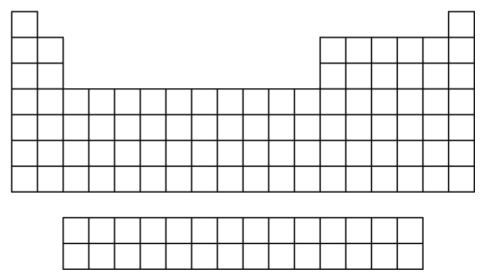
\includegraphics[width=\linewidth]{../images/blank-periodictable}
%     \end{figure}
% \end{minipage}
